\section{Raw data}
The simulations took varying amounts of time to complete with some of the longer
programs taking 30-40 hours per thread version. Therefore, it took around a week
before the majority of the data was available, with only the \texttt{volrend} 
program runs still going; they seemed to take around 70 hours each. Excluding 
the \texttt{volrend} benchmark, there was 320 simulations to retrieve: 8 
benchmarks $\times$ 8 big.LITTLE configurations $\times$ 5 different number of 
threads. A total of 120GB of raw text data was accumulated from the programs 
excluding \texttt{volrend}, with each \texttt{stats.txt} file typically being 
between 2.5-4 million lines long. However, as most of the stats recorded by the 
simulator are much more detailed than what could be recorded and used by using 
PMUs, the extracted data size is much smaller.

    \subsection{Problems encountered}
        \subsubsection{Network outage}
        As mentioned, the \texttt{volrend} benchmark took significantly longer 
        than the other programs being run on the simulator. Unfortunately, this 
        meant that it was still running during the University-wide network 
        outage that occurred on the 9\textsuperscript{th} of May. Although the 
        vast majority of the University's network infrastructure was restored 
        quickly, it took a while before access to the cluster was 
        re-established. Additionally, it seems the network outage affected the 
        \texttt{tmux} sessions that were being used to run the benchmarks, 
        despite them being local to each micro server. As a result the 
        \texttt{volrend} data was incomplete and was inaccessible until shortly 
        before the deadline. Because of these issues, the \texttt{volrend} data 
        was not used for the project.
    
        \subsubsection{Benchmark crashes}
        Each bootscript was set to print the line ``\texttt{Benchmark done, 
        exiting simulation.}'' once the benchmark had returned. This allowed me 
        to easily be able to tell if the runs had completed successfully, in 
        case some of them crashed. Unfortunately, once the data was downloaded 
        from the various micro servers and assembled in one place, it became 
        apparent that despite running for a long time, a lot of the benchmarks 
        seemed to have crashed near the end of their execution. By counting the 
        number of times the ``\texttt{Benchmark done}[...]'' line occurred, the 
        following completion ratios were obtained:
        \begin{table}[H]
            \centering
            \begin{tabular}{l|c|c|r}
                \textbf{benchmark} & \textbf{n\_finished} & \textbf{n\_crashed} 
                & \textbf{completion\_ratio} \\
                \hline
                \texttt{barnes} & 20 & 20 & 50.0\% \\
                \texttt{fmm} & 9 & 31 & 22.5\% \\
                \texttt{ocean-contiguous\_partitions} & 13 & 27 & 32.5\% \\
                \texttt{ocean-non\_contiguous\_partitions} & 0 & 40 & 0.0\% \\
                \texttt{radiosity} & 13 & 27 & 32.5\% \\
                \texttt{raytrace} & 8 & 32 & 20.0\% \\
                \texttt{water-nsquared} & 9 & 31 & 22.5\% \\
                \texttt{water-spatial} & 5 & 35 & 12.5\% \\
            \end{tabular}
            \caption{Completion ratios for the various benchmarks}
        \end{table}
        As mentioned earlier, most of the crashed benchmarks seem to have 
        crashed towards the end of their execution. The exception is the 
        \texttt{ocean-non\_contiguous\_partitions}, which seems to have crashed 
        within milliseconds of starting. When plotting the power usage of the 
        cores for some of the benchmarks (Appendix \ref{ch:power-plots}), it 
        becomes clear that the crashes occurred very near the end of the 
        benchmark runs. If one were to look purely at the plots, it would be 
        difficult to say which crashed and which did not based on their power 
        consumption and time taken. Therefore, the data from the crashed 
        benchmarks was kept in the final data set.
    
\section{Data extraction}
    \subsection{Mapping gem5 stats to PMU events}
    In order to keep the data as realistic as possible so as to potentially be 
    able to implement the results on real hardware, only data entries which 
    could be obtained through the PMUs were kept. Not all data that the PMUs 
    are capable of recording is available in the gem5 stats. For example, while 
    there is a detailed overview of what amount of data was sent over the 
    memory bus, how many packets were used, and which parts sent them, there 
    does not seem to be an equivalent of the PMU event \texttt{0x19}: ``Bus 
    access''. Some stats also require slightly greater care to extract, e.g. 
    the number of architecturally executed/committed instructions (PMU event 
    \texttt{0x08}) is recorded as \textsf{[...]commit.committedInsts}'' for 
    CPUs in the big cluster but simply as ``\textsf{[...].committedInsts}'' for 
    CPUs in the LITTLE cluster. Since the stats blocks in the files are often 
    1000s of lines, these subtleties are easy to miss when skimming through the 
    stats files. Fortunately, most of the PMU events have a clear, direct 
    equivalent in the stats file. The complete map between stats and PMU events 
    is:
    \begin{table}[H]
        \centering
        \begin{tabular}{r|c|l}
            \textbf{gem5 stat} & \textbf{PMU event} & \textbf{description} \\
            \hline
            \textsf{branchPred.BTBLookups} & \texttt{0x12} & Predictable branch
                speculatively executed \\ 
            \textsf{committedInsts} & \texttt{0x08} & Instruction 
                architecturally executed \\
            \textsf{branchPred.condIncorrect} & \texttt{0x10} & 
            \begin{tabular}[c]{@{}l@{}}Mispredicted or
                not predicted branch\\ speculatively executed\end{tabular} \\
            \textsf{numCycles} & \texttt{0x11} & Cycle {[count]} \\
            \textsf{icache.overall\_accesses::total} & \texttt{0x14} & L1
                instruction cache access \\
            \textsf{dcache.overall\_accesses::total} & \texttt{0x04} & L1 data
                cache access \\
            \textsf{dcache.writebacks::total} & \texttt{0x15} & L1 data cache
                Write-Back \\
            \textsf{l2.overall\_accesses::total} & \texttt{0x16} & L2 data cache
                access \\
            \textsf{l2.writebacks::total} & \texttt{0x18} & L2 data cache
                Write-Back \\
        \end{tabular}
        \caption{Mapping between gem5 stats and PMU events (in order of 
        occurrence in the stats files)}
    \end{table}

    The branch prediction stats were somewhat challenging to derive. Initially,
    I believed that the ``\textsf{branchPred.condPredicted}'' corresponded to 
    the PMU event for speculatively executing a branch. However, looking 
    through the source code, I discovered that the stat is always incremented 
    \textit{before} predicting if the branch is taken or not (Figure 
    \ref{subfig:bp-condpredicted-wrong}). Additionally, I discovered that the 
    PMU registered to the gem5 Simulator seems to get incremented each time the 
    branch predictor is used instead of each time a ``[p]redictable branch [is] 
    speculatively executed'' (Figure \ref{subfig:bp-lookups-wrong}). The 
    \textsf{BTBLookups} stat is the only viable option, as it is incremented 
    each time a conditional branch (not a return address) is predicted as taken 
    (Figure \ref{subfig:bp-btblookups-correct}).
    \begin{figure}[H]
        \centering
        \begin{subfigure}{0.55\linewidth}
            \centering
            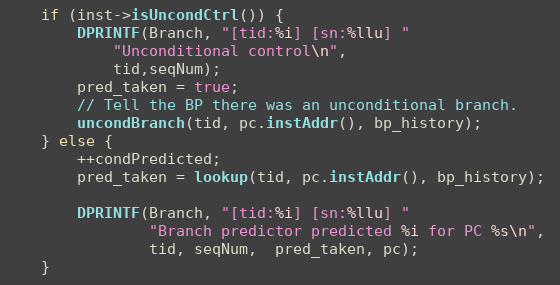
\includegraphics[width=\textwidth]{screenshots/br-pred/br-pred-pmu-0x12-condPredicted-src.png}
            \caption{\texttt{condPredicted} increments before the prediction}
            \label{subfig:bp-condpredicted-wrong}
        \end{subfigure}
        \begin{subfigure}{0.55\linewidth}
            \centering
            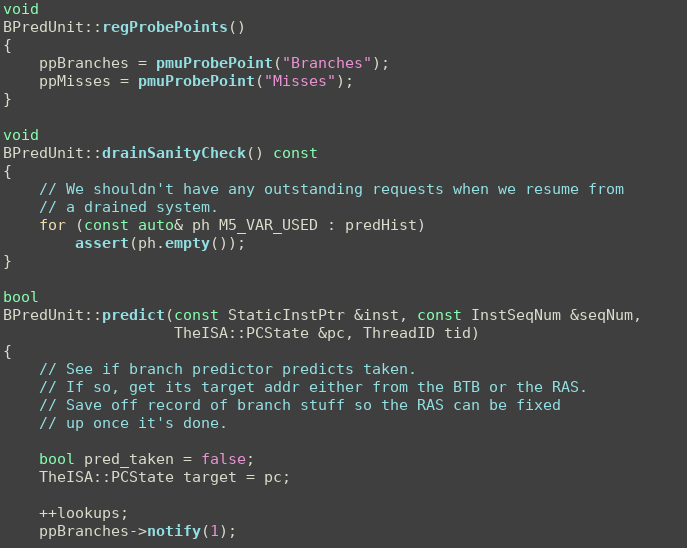
\includegraphics[width=\linewidth]{screenshots/br-pred/br-pred-pmu-0x12-maybe.png}
            \caption{\texttt{lookups}, which is wired up to the gem5 PMU, seems
                     to get incremented on each branch predictor access}
            \label{subfig:bp-lookups-wrong}
        \end{subfigure}
        \begin{subfigure}{0.55\linewidth}
            \centering
            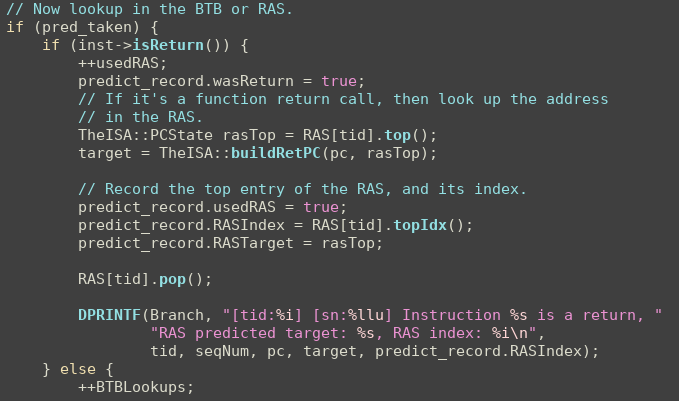
\includegraphics[width=\linewidth]{screenshots/br-pred/br-pred-pmu-0x12-if-pred-taken.png}
            \caption{\texttt{BTBLookups} is incremented if the branch was a
                     conditional branch \emph{and} it was predicted as taken}
            \label{subfig:bp-btblookups-correct}
        \end{subfigure}
        \caption{The source C++ code of various branch predictor stats}
    \end{figure}
    For branch mispredictions, the \textsf{condIncorrect} fortunately seems to 
    be correct and (according to the code comments) only get incremented when 
    the branch was discovered to be mispredicted.
    \begin{figure}[H]
        \centering
        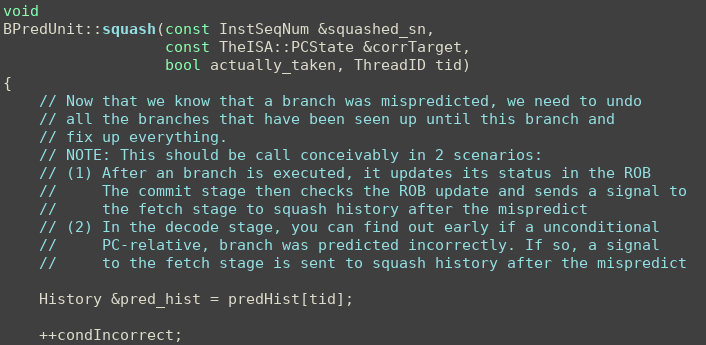
\includegraphics[width=0.55\linewidth]{screenshots/br-pred/br-pred-pmu-0x10-condIncorrect-src.png}
        \caption{The C++ code confirms that \texttt{condIncorrect} stat 
                 monitors branch mispredictions}
    \end{figure}

    \subsection{The \texttt{data-aggregate.py} script}
    Having derived which PMU events could be extracted from the gem5 stats, I 
    wrote a script which would scrape each of the many stat files, extract, and 
    aggregate the stats into a single file. The script takes the top-level 
    directory which contains the benchmark output directories as structured 
    through the experimental setup. Since the path to each stats file contains 
    information as to what benchmark, which setup, and how many threads were 
    used, this information is collected when going down the directory 
    structures. For each stat block in the stats file, a line in a CSV-file is 
    then created. Each line contains the information stored in path/directory 
    names, a time increment in the simulation, all the PMU stats, and the power 
    stats. It is possible to specify the name of the output file through the 
    \texttt{--output} flag.
    
    Running the script on the 120GB of collected data produced a CSV file of 
    101MB. This is still a lot of text, but it is also much more manageable than
    the 120GB of full-detail data.

\section{Data Processing}
    \subsection{Pre-processing}
    The extracted data needed to be pre-processed before it could be used. For 
    the comparisons between PMU measurements to be fair, the measurements are 
    divided by the number of cycles. Each time slice of 1ms can contain a 
    different number of cycles simulated, due to varying number of stalls or 
    less activity on the core(s), so by dividing the PMU measurements by the 
    number of cycles simulated that time slice, the comparisons become fairer 
    than comparing the time slices directly. The static and dynamic power 
    measurements were added up to be one `\texttt{total\_power}' measurement.
    
    By creating a multi-index dataframe ordered by benchmark name, big.LITTLE 
    configuration, number of threads, time slice, cluster, and CPU, the data 
    can then be added up over time, resulting in one entry per benchmark, 
    configuration, number of threads, cluster, and CPU which can be easily 
    compared to other instances and/or other benchmarks in order to determine 
    which setup(s) were best in terms of power savings. To be able to compare 
    the total power of the different runs, the power was normalised using 
    Min-Max Feature scaling. This fits the measurements into a range between 0 
    and 1 inclusive, based on the minimum and maximum values in the dataset, 
    which then makes the power measurements easier to plot and compare since 
    all the records will at most have a power value of 1, whilst also 
    maintaining the relative size differences. The scaling was done using the 
    \texttt{minmax\_scale} function from Scikit-Learn's 
    \cite{pedregosa_scikit-learn_2011} \texttt{preprocessing} module.
    
    \subsection{Predicting and Plotting}
    Since it was too late to try to implement a new scheduler, we instead 
    decided to look at whether the recorded data could show that a more 
    power-efficient schedule existed. The idea was as follows:
    \begin{enumerate}
        \item Select a benchmark that will be arriving as a new program.
        \item Get the PMU data by `running' it on a stock big.LITTLE
              configuration. This should reveal some details about the program
              and can simply be looked up since we have all the runs already.
        \item Based on the PMU data, predict what benchmark is the most similar
              by looking at data which does not contain any information about 
              the benchmark run, for some definition of `similar'.
        \item Find the optimal big.LITTLE configuration for that benchmark, for
              some definition of `optimal', and get its results.
        \item `Run' the actual benchmark on the configuration and measure/look
              up the actual results.
        \item Compare the predicted and actual results, along with a baseline.
    \end{enumerate}

    To keep the predictions and comparisons simple, only datapoints from 
    configurations where the number of threads of the benchmark was equal to 
    the number of cores available were kept. The rationale was that this 
    optimised the usage of the configuration and so allowed us to see the 
    fastest the benchmark could perform on that setup, allowing us to see if and
    how the benchmark scaled.
    
    We decided to use Nearest-Neighbours with Euclidean Distance to determine 
    similarity. This was done using the default settings for the 
    \texttt{KNearestNeighborsClassifier} in Scikit-Learn's 
    \cite{pedregosa_scikit-learn_2011} \texttt{neighbors} module. The stock 
    configuration was set to be a 2 big 2 LITTLE configuration because it was a 
    configuration which seemed to be somewhere in the middle, hopefully 
    allowing for balanced predictions in either direction.
    
    The predictions were done, leaving each benchmark out in turn and 
    retraining the module each time. Since the model returned multiple 
    predictions, one for each core in the stock configuration, these were 
    treated as votes and the benchmark with the most votes was selected for 
    comparison. Based on which benchmark was predicted to be most similar, the 
    optimal configuration for that benchmark was then found by minimising all 
    the number of cycles and amounts of power consumed by the setup for the most
    most similar benchmark. To compare across different configurations, which 
    have a different number of cores to compare, the power was accumulated and 
    only the highest number of cycles per cluster was kept. This was done since 
    power consumption is additive, and the largest number of cycles will 
    indicate the last point at which the final thread of the benchmark finished.
    It was possible to get more than one configuration back if they were equally
    optimal, however no such situation occurred.
    
    Taking the most similar benchmark and its optimal configuration, the data 
    from the corresponding run with the number of threads equal to the total 
    number of cores) was retrieved, as was the data from the actual benchmark on
    the predicted benchmark's actual configuration. Initially, the baseline was 
    to pick a random configuration and compare with the run on this. However, 
    due to the small number of possible configurations, each was enumerated 
    instead so as to be able to compare all the possible setups.
    
    For each baseline, a plot showing the number of cycles and amount of power 
    for the big and LITTLE clusters was created. These plots allowed me to 
    easily spot and compare the performance of the various benchmarks and 
    configurations. The name of the benchmark predicted to be the most similar
    was put next to the bars showing its performance, for clarity.
    
\section{Analysis}
    \subsection{Plots and observations}
    The behaviour of the Nearest-Neighbours model for the different benchmarks 
    is largely identical. It seems to always put the \texttt{barnes} benchmark
    as the most similar, and the optimal configuration in this case is always
    4b4L. The benchmark most similar to \texttt{barnes} seems to be the 
    \texttt{fmm} benchmark, with the 1b1L configuration being the most optimal.
    \begin{figure}[H]
        \centering
        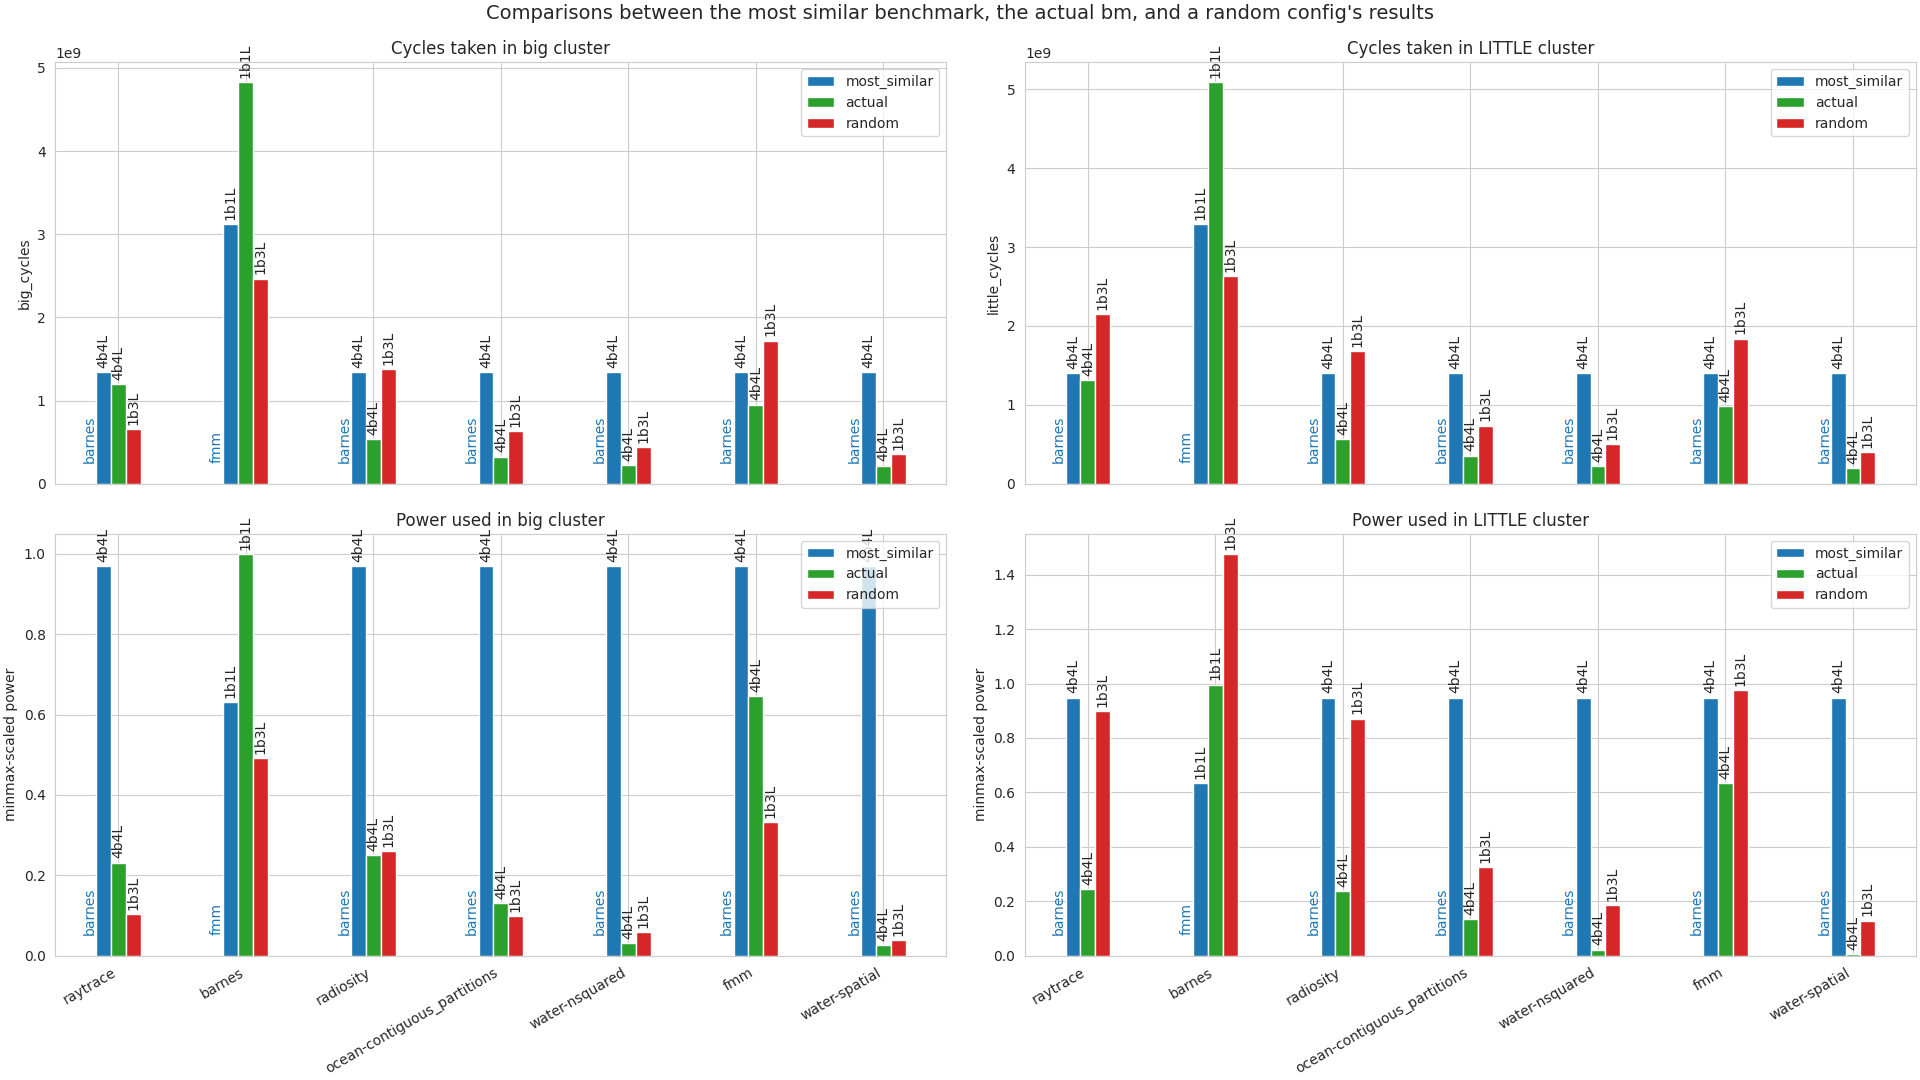
\includegraphics[width=\textwidth]{pred-plots/stock-2b2L/rand-1b3L.png}
        \caption{Performance comparisons using 1b3L as the baseline}
        \label{fig:s-2b2L-r-1b3L}
    \end{figure}
    
    Looking at the plots (note the y-axis for cycles is in giga, i.e. 
    \textsf{1e9}, cycles), it becomes apparent that the trade-offs are there, 
    but that the model has not been very successful in picking up on them, or 
    perhaps the method for finding the optimal configuration could be improved.
    When comparing the plots with a 1b3L baseline (Figure 
    \ref{fig:s-2b2L-r-1b3L}) with the plots with a 2b2L baseline(Figure 
    \ref{fig:s-2b2L-r-2b2L}), i.e. sticking with the stock configuration, we can
    see that swapping a little core for a big core marginally improves 
    performance for certain benchmarks' LITTLE clusters (e.g. \texttt{raytrace})
    with a slight decrease in performance (increased number of cycles taken) on 
    the big clusters. However, the big core consumes much more power, taking 
    nearly as much power in the \texttt{barnes} scenario as the 1b1L 
    configuration.
    \begin{figure}[H]
        \centering
        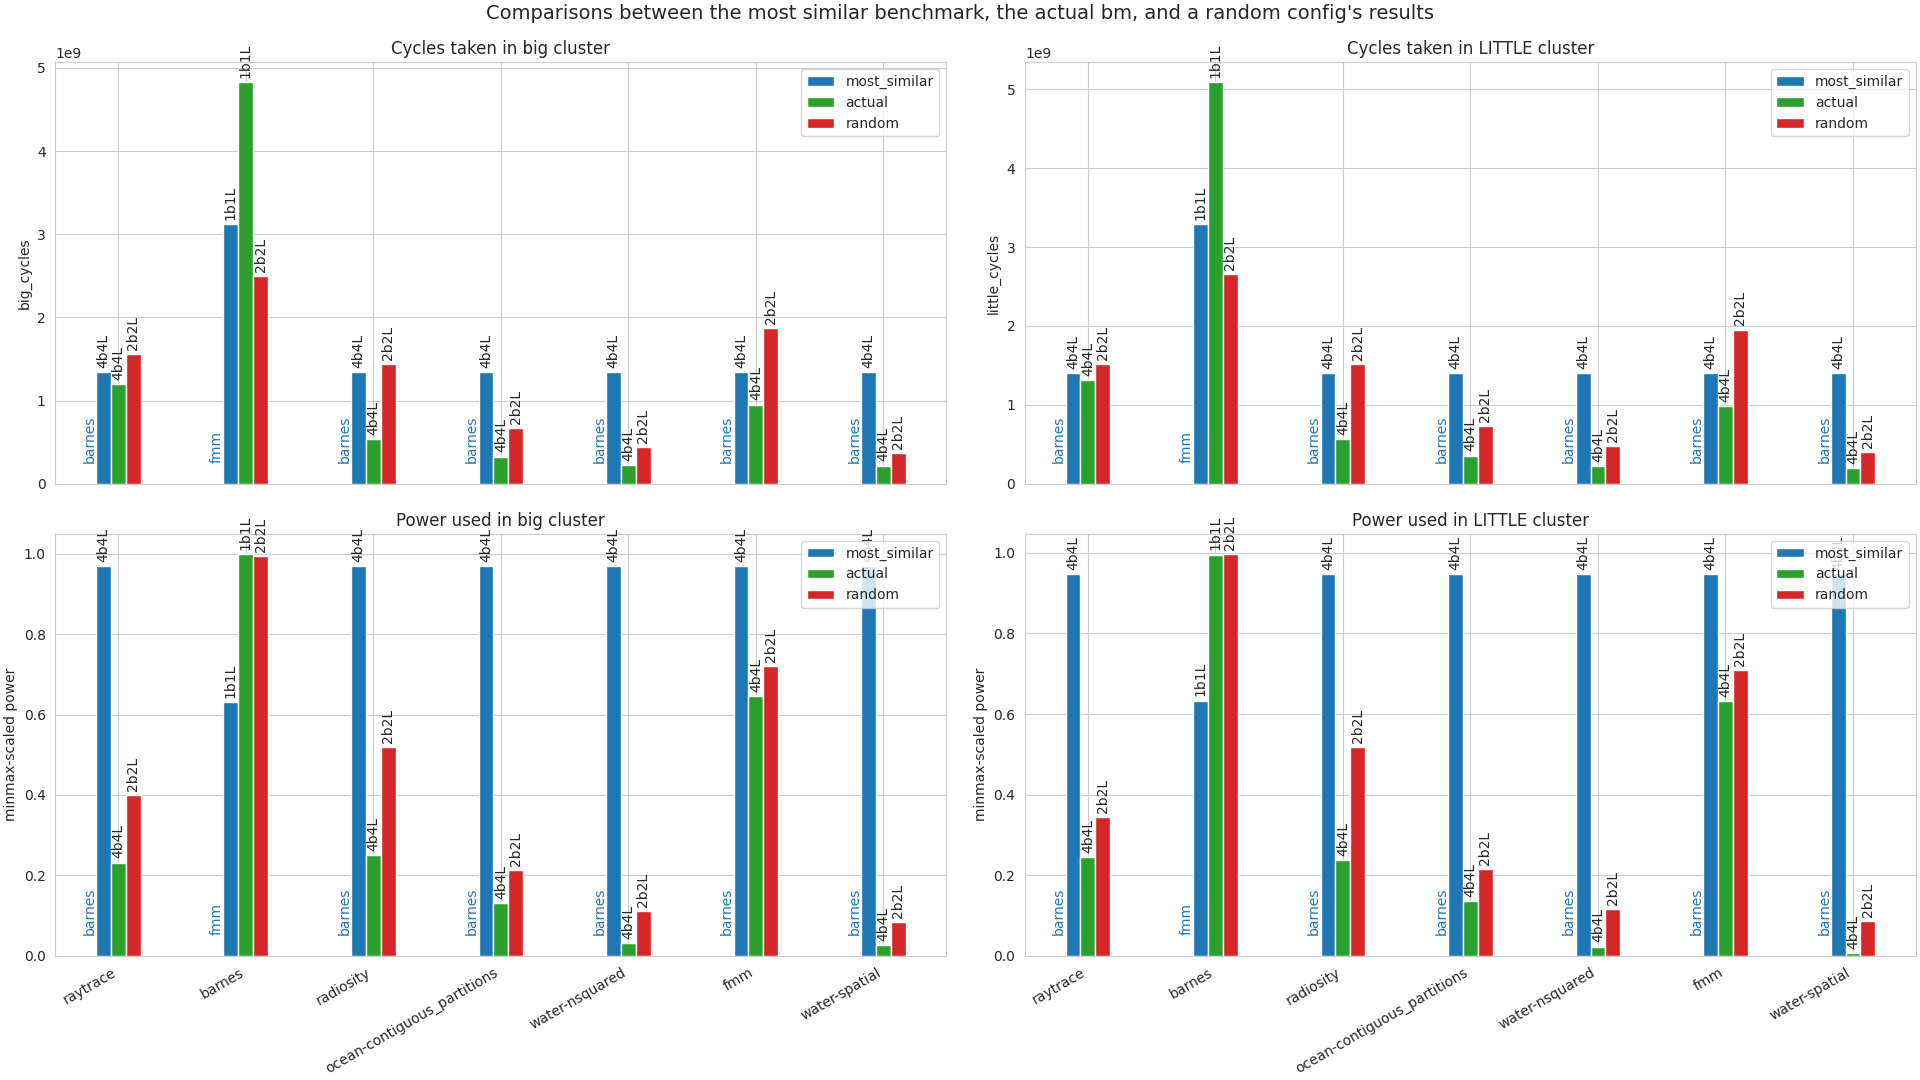
\includegraphics[width=\textwidth]{pred-plots/stock-2b2L/rand-2b2L.png}
        \caption{Performance comparisons using 2b2L as the baseline}
        \label{fig:s-2b2L-r-2b2L}
    \end{figure}

    Looking further at the plots with a 3b1L baseline (Figure 
    \ref{fig:s-2b2L-r-3b1L}, both \texttt{raytrace} \texttt{radiosity} seem to 
    improve performance and power on the LITTLE clusters, taking longer on the 
    big cluster, with the other benchmarks increasing or decreasing by smaller 
    amounts. Similar to the switch between 1b3L and 2b2L, adding the extra big
    core increases power consumption a lot.
    \begin{figure}
        \centering
        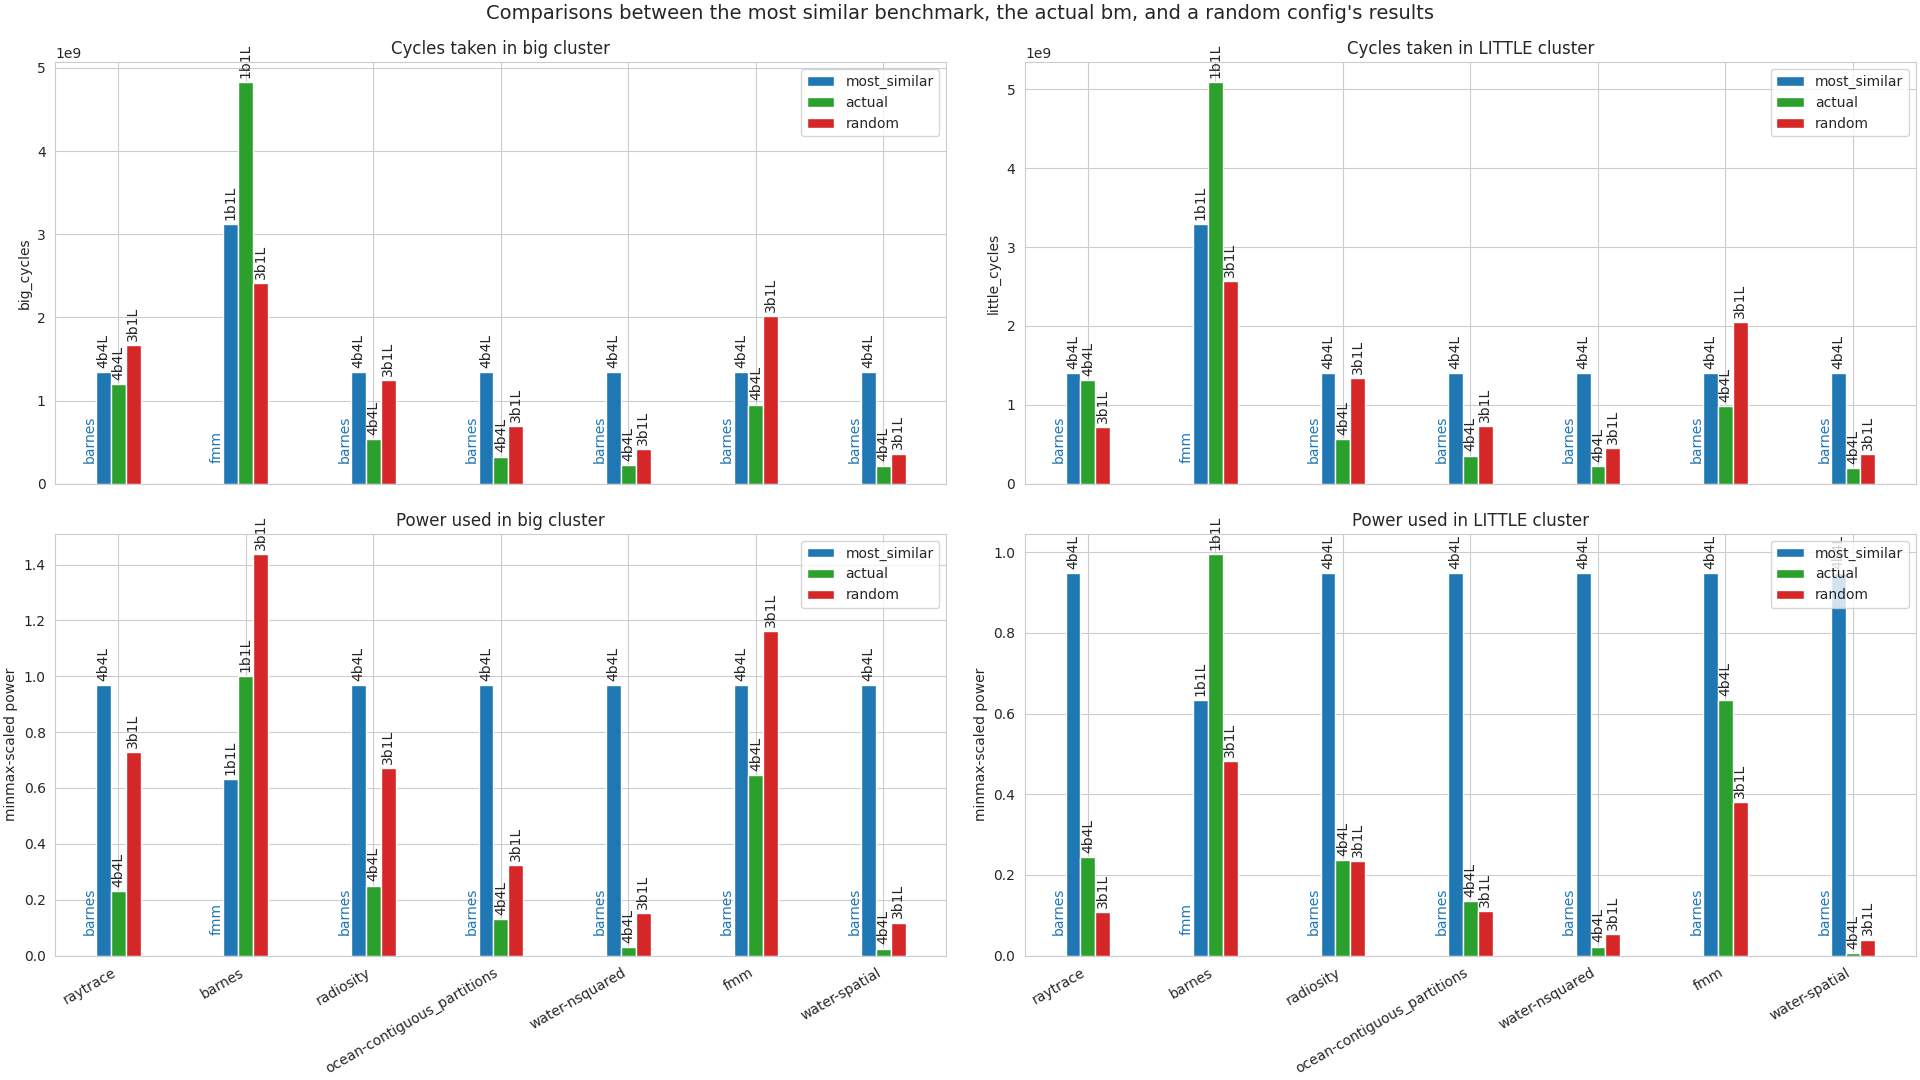
\includegraphics[width=\textwidth]{pred-plots/stock-2b2L/rand-3b1L.png}
        \caption{Performance comparisons using 3b1L as the baseline}
        \label{fig:s-2b2L-r-3b1L}
    \end{figure}
    
    It should be noted that the normalisation, or perhaps the result retrieval 
    function, seems to have not quite worked and as a result, the power plots 
    corresponding to the cluster with 3 cores in the 3b1L and 1b3L 
    configurations exceeds the normalised 0-1 scale. This does not happen with 
    the other plots, so it could be that the unbalanced configuration causes a 
    problem. Unfortunately, I was able to narrow down this bug.
    
    \subsection{Evaluating the prediction results}
    The differences between the predicted results and the actual results are 
    quite large. With most of the benchmarks, the predicted power consumption is
    many times greater than the actual performance, both on the big and LITTLE 
    clusters. While predicting the power consumption to be higher than it turns 
    out to be is likely better than predicting it to be too low, it does show 
    that the model is very imprecise, possibly due to lack of data.
    
    Interestingly, the tactic of always going with 4b4L does not seem bad when 
    looking at the overall performance. Each time a different configuration 
    manages to do better on one cluster, it seems to come at a cost on the 
    other cluster. This is likely due to 4b4L requiring more power in theory, 
    but finishing the benchmarks so much faster that it does not matter.
    
    \subsection{Using other stock configurations}
    In order to improve performance of the model, more data could be supplied. 
    One way of doing this would be to `run' the arriving benchmark on more than 
    one stock configuration and using the results from all the stock 
    configurations as input when predicting the most similar. I tried using 
    pairs of configurations: 2b2L+1b3L, 2b2L+4b4L, 3b1L+1b3L. The idea was that
    the change in balance between the configurations would lead to a change in 
    predictions as there were `examples' of which cores affected what. However, 
    when plotted, the results were identical. Some examples can be seen in 
    Appendix \ref{ch:multis-pred-res}. The complete set of plots can be found in
    the \texttt{pred-plots} directory.
